\documentclass{article}

\usepackage{minted}
\usepackage{csquotes}
\usepackage[backend=biber]{biblatex}
\usepackage[T1]{fontenc}
\usepackage[polish]{babel}
\usepackage[utf8]{inputenc}
\usepackage{graphicx}



\author{Mateusz Muśko}
\title{Dokumentacja Projektu KCK cz. I}

\begin{document}

\maketitle
\tableofcontents

\section{Opis projektu}

\paragraph{}

Projekt ten ma na celu ułatwienie agregację informacji na temat zdrowia oraz sytuacji związanej z obecnie panującym wirusem SARS-CoV-19. Zbiera on informacje ze zdefiniowanych wcześniej stron i udostępnia je użytkownikowi w skompresowanej formie, bez reklam oraz innych "zapychaczy" miejsca na ekranie

\section{Opis funkcjonalności}

\paragraph{}
Aplikacja ma dwa główne zadania:
\begin{itemize}
    \item Pobierać oraz wyświetlać artykuły ze zdefiniowanych wcześniej stron
    \item Dostarczać danych statystycznych na temat wirusa SARS-CoV-19
\end{itemize}
Dostarcza również podstawowe funkcje konfiguracyjne takie jak zmiana kolorów powiadomień

\section{Instrukcje}

\subsection{Instrukcja instalacji}

\paragraph{}
Do zainstalowania aplikacji potrzebna jest podstawowa obsługa terminalu systemowego

\paragraph{}
Aby zainstalować aplikację należy rozpakować archiwum app.zip w miejscu wybranym przez użytkownika.
Archiwum to powinno zawierać:
\begin{itemize}
    \item sites - przechowywane są tutaj pobrane artykuły
    \item app.py - odpowiada za wygląd aplikacji
    \item CovidStatistics.py - narzędzie do pobierania i obróbki danych statystycznych
    \item main.py - plik główny
    \item News.py - narzędzie do pobierania i obróbki artykułów
    \item script.bat - tworzy potrzebne katalogi i pliki konfiguracyjne (windows Only)
\end{itemize}
Aczkolwiek przed uruchomieniem aplikacji należy sprawdzić czy zainstalowany został wcześniej interpreter języka Python, 
aby to zrobić w terminalu wpisujemy komendę:

\begin{minted}[frame=lines]{bat}
C:\Users> python --version
Python 3.7.4
\end{minted}

Po wykonaniu komendy powinniśmy zobaczyć wersję zainstalowanego interpretera. Jeżeli tak się nie stało musimy pobrać python'a ze strony:\\
https://www.python.org/downloads/

\paragraph{}
Następnie musimy zainstalować moduły języka python potrzebne do działania aplikacji,
 używamy do tego narzędzia pip, a więc musimy sprawdzić czy jest ono zainstalowane, (jeżeli korzystasz z języka Python w wersji 3.4 bądź wyższej pip powinien być zainstalowany):

\begin{minted}[frame=lines]{bat}
C:\Users> pip --version
pip 19.2.3 from C:\Users\..\lib\site-packages\pip (python 3.7)
\end{minted}

Tak samo jak w przypadku interpreter powinniśmy zobaczyć wersję narzędzia pip. W razie problemów odsyłam do dokumentacji języka Python:\\ 
https://docs.python.org/3/using/index.html

\pagebreak
A więc przejdźmy do zainstalowania modułów robimy to za pomocą komendy:

\begin{minted}[frame=lines]{bat}
C:\Users> pip install nazwa_modułu
\end{minted}

W naszym przypadku będą to komendy:
\begin{minted}[frame=lines]{bat}
C:\Users> pip install npyscreen
C:\Users> pip install newspaper
C:\Users> pip install bs4
C:\Users> pip install requests
\end{minted}

Gdy zainstalujemy potrzebne moduły możemy przejść do uruchomienia aplikacji. 
Gdy znajdujemy się w ścieżce do której wypakowaliśmy archiwum, robimy to za pomocą komendy:

\begin{minted}[frame=lines]{bat}
C:\Users> python main.py
\end{minted}


\subsection{Instrukcja konfiguracji}

W przypadku tej aplikacji konfiguracja nie powinna być konieczna, gdyż wszystkie foldery oraz pliki powinny znajdować się już w archiwum.
Natomiast jeżeli po rozpakowaniu archiwum wciąż mamy błąd z brakującymi plikami, należy uruchomić script.bat służy on do odtworzenia ścieżek z plikami oraz folderów.
Jeżeli natomiast nie mamy w archiwum któregoś z plików .py wylistowanych w Podpunkcie 3.1 tej dokumentacji należy skontaktować się z twórcą aplikacji 

\pagebreak

\subsection{Instrukcja użytkownika}

Po pierwszym uruchomieniu aplikacji zobaczymy ekran główny\\ \\
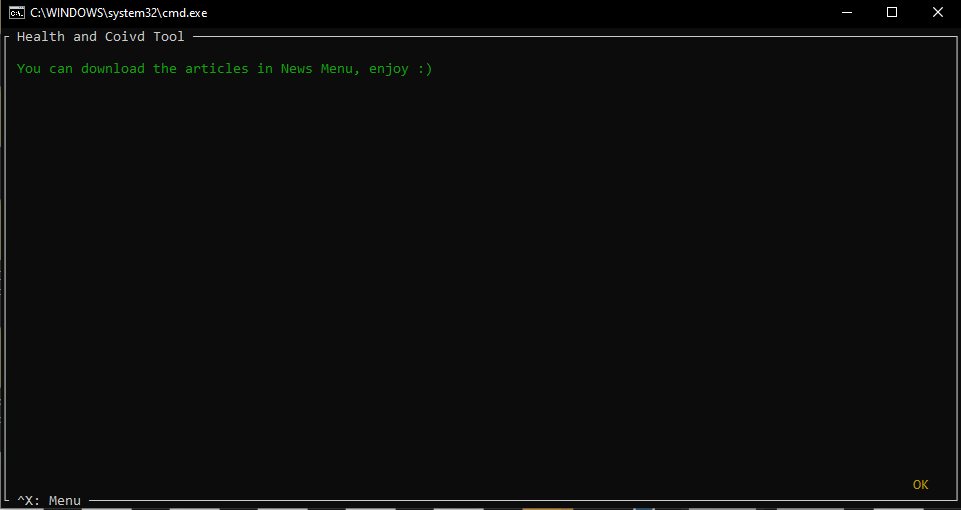
\includegraphics[width=\textwidth]{images/main_screen_first_run.png}

Oznacza to że aplikacja nie pobrała jeszcze żadnych artykułów do wyświetlenia. Aby to zrobić otwieramy Menu kombinacją klawiszy Ctrl + X,
następnie wybieramy za pomocą strzałek pozycję News i zatwierdzamy enterem, możemy to również zrobić wciskając klawisz "1"

\paragraph{}
Po wybraniu tej opcji powinniśmy zobaczyć ekran z tekstem "There is no articles to view". Po raz kolejny otwieramy Menu: \\
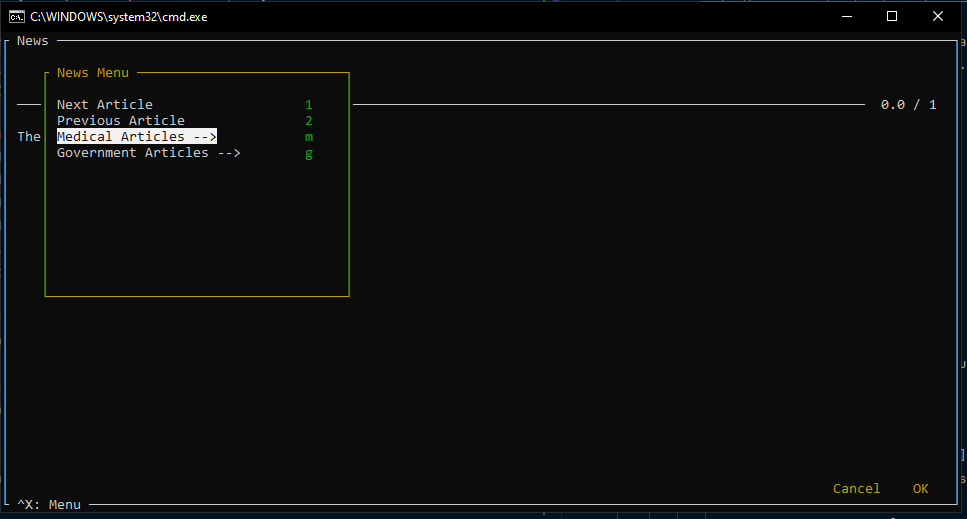
\includegraphics[width=\textwidth]{images/news_screen_menu.png}

\pagebreak

\paragraph{}
Następnie wybieramy jedną z opcji Medical Articles, bądź Government Articles, powinno nam się ukazać podmenu z dwiema opcjami:\\
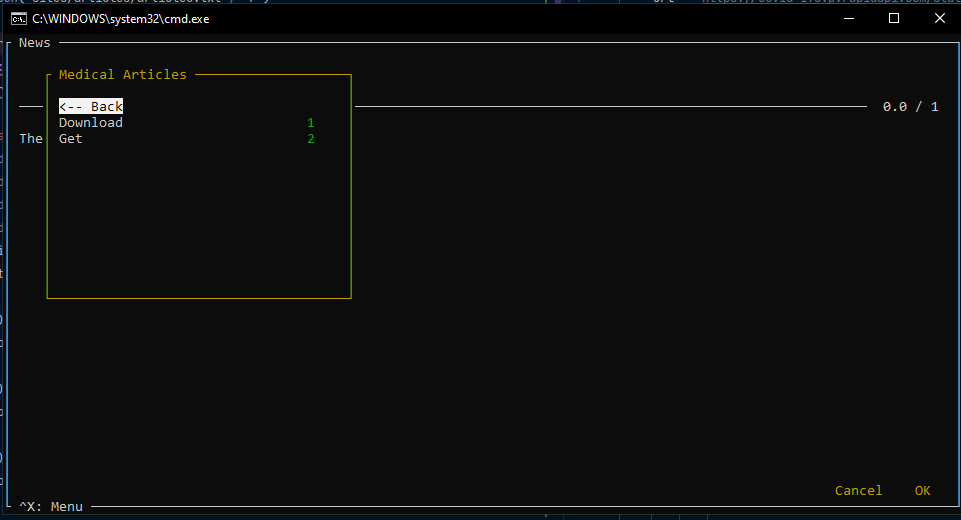
\includegraphics[width=\textwidth]{images/news_screen_sub_menu.png}

\begin{itemize}
    \item Opcja Download służy do pobrania artykułów na dysk i zapisanie ich w plikach UWAGA!! Może to zająć chwilę w zależności od ilości artykułów na stronie
    \item Natomias Get pobiera artykuły zapisane na dysku oraz przygotowuje do wyświetlenia na ekranie
\end{itemize}

Po wybraniu opcji Download powinniśmy zobaczyć komunikat:\\
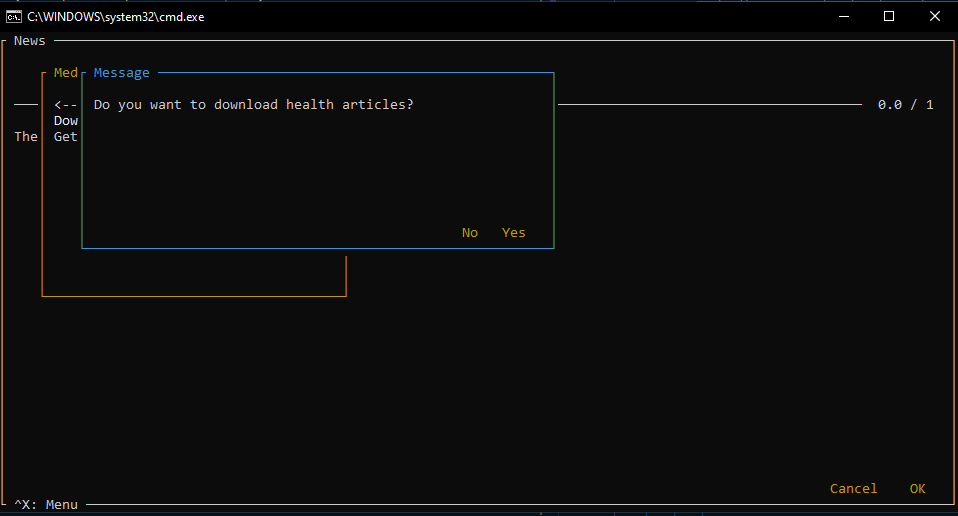
\includegraphics[width=\textwidth]{images/download_articles.png}
należy wybrać opcję YES gdy chcemy aby artykuły zostały zapisane na dysku, lub NO gdy nie chcemy tego robić.\\

\pagebreak
No dobrze, ale gdy wciśniemy YES i zniknie komunikat 'Be patient it might take some time :)' nic się nie wyświetla,
to dlatego że musimy użyć jeszcze opcji Get dla odpowiedniej kategorii artykułów , znów otwieramy Menu ale tym razem zamiast Download używamy opcji Get.
Po zatwierdzeniu powinniśmy zobaczyć pierwszy artykuł:\\

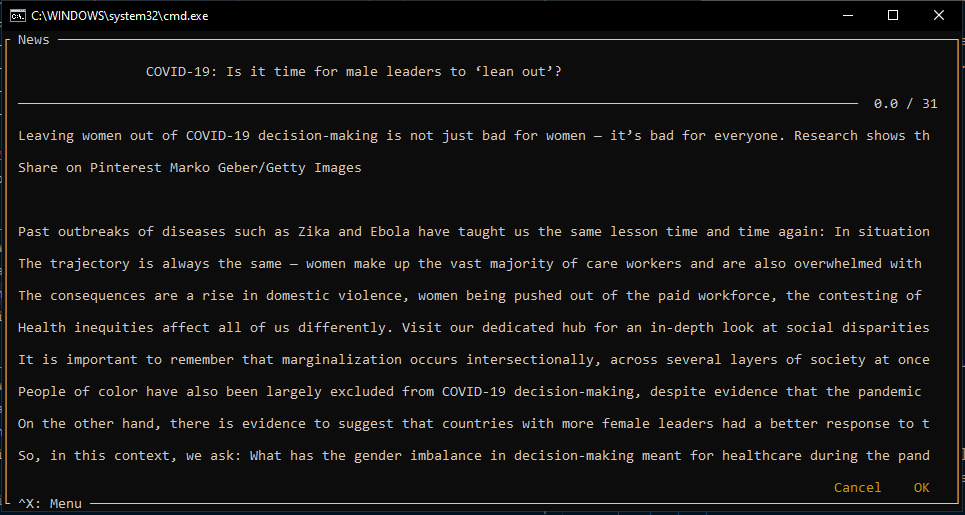
\includegraphics[width=\textwidth]{images/first_article.png}\\

Artykuł przewijamy strzałkami Góra i Dół oraz aby przejść do następnego artykułu należy wybrać odpowiednią opcję z menu kontekstowego.

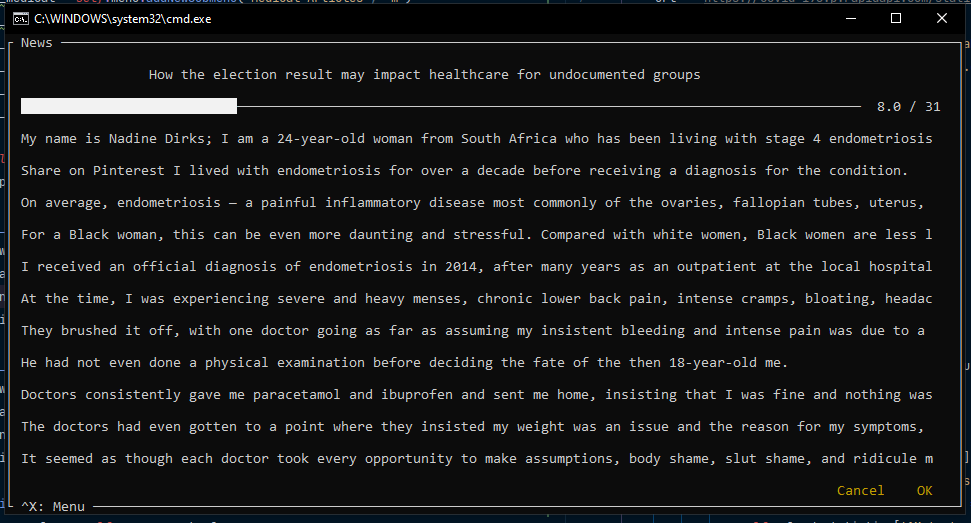
\includegraphics[width=\textwidth]{images/next_article.png}

Oto następny artykuł, zauważmy że nad artykułem znajduje się pasek który podowiada w ile artykułów już przeczytaliśmy

Aby wyjść z tego widoku należy wcisnąć ENTER i wybrać Cancel w prawym dolnym rogu


\section{Zagadnienia projektowe}

Podczas tworzenia tej aplikacji jednym z największych problemów było przedstawienie aplikacji w minmalistyczny i funkcjonalny sposób tak,
aby użytkownik nie czuł się zagubiony podczas korzystania z aplikacji. Również ważnym aspektem było aby aplikacja ta mogła działać na większości terminali oraz
ekranów. Podczas pisania aplikacji natknąłem się na problem wyświetlania większej ilości znaków  niż pozwalał na to terminal. Zauważyłem to dopiero gdy postanowiłem przetestować aplikację na mniejszym monitorze
,ponieważ aplikacja była programowana na monitorze o rozdzielczości 2560x1440 po zmniejszeniu jej terminal nie był w stanie wyświetlić długich linii tekstu i aplikacja wyrzucała błąd.
Kolejnym problemem jest zaprogramowanie aplikacji tak aby była jak najbardziej intuicyjna, co w dobie gdy większość aplikacji ma graficzne interfejsy
jest nie lada wyzwaniem, ponieważ użytkownikom prościej korzysta się z takich interfejsów gdyż są oni z nimi bardziej zaznajomieni i interfejsy te pozwalają na większą swobodę, oraz posiadają większe możliwości.


\section{Wnioski}

Projektowanie interfejsu tekstowego do aplikacji w dzisiejszych czasach wydaje się przestarzałym rozwiązaniem. Jednak w pewnych sytuacjach
interfejsy tekstowe mają zdecydowaną przewagę nad graficznymi, gdyż pozwalają użytkownikowi skupić się na tym co najważniejsze. W przypadku tej aplikacji
są to treści artykułów które użytkownik chce przeczytać oraz dane statystyczne związane z obecną pandemią. Użytkownik nie jest rozpraszany 
reklamami bądź innymi "zapychaczami" miejsca na ekranie, co pozwala na szybkie oraz łatwe odnalezienie potrzebnych informacji i danych. Jest to
jedna z przyczyn dla których informatycy wolą pracować w środowiskach z interfejsem tekstowym, kolejną zaletą interfejsów tekstowych jest ich wysoki poziom
kompatybilności, gdyż w z decydowanej większości przypadków urządzenia przez nas spotykane na pewno wyświetlają tekst co pozwala na implementację
interfejsów tekstowym praktycznie wszędzie

\subsection{Samoocena}
Uważam, że w przypadku tego projektu wiele rzeczy można jeszcze poprawić oraz rozbudować rozbudowanie konfiguracji aplikacji. Ze względu na czynniki niezależne od mojej osoby
nie udało mi się wyciągnąć pełni potencjału z pomysłu jaki sobie narzuciłem. Jest to dobra aplikacja jednak daleka od ideału. Jeżeli miałbym sobie wystawić ocenę
było by to coś w granicach 3,5 - 4.

\end{document}